\documentclass[border=2pt]{standalone}
\usepackage{times}
\usepackage{amsmath,amssymb}
\usepackage{tikz}
\usetikzlibrary{arrows.meta,calc,positioning}
\begin{document}
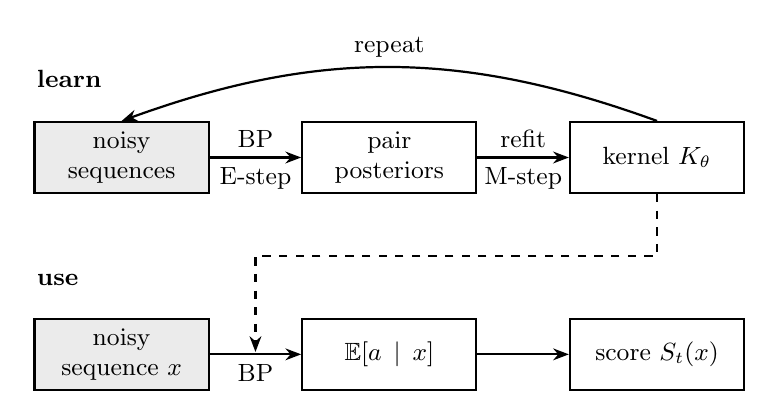
\begin{tikzpicture}[
    box/.style={draw,thick,align=center,font=\small,minimum height=9mm,inner sep=3pt,text width=2.0cm},
    data/.style={box,fill=black!8},
    arr/.style={-{Stealth[length=2mm]},thick},
    lab/.style={font=\small,align=center}]
  \node[font=\small\bfseries,anchor=west] at (-1.2,1.0) {learn};
  \node[data] (d) at (0,0) {noisy\\ sequences};
  \node[box] (p) at (3.4,0) {pair\\ posteriors};
  \node[box] (k) at (6.8,0) {kernel $K_\theta$};
  \draw[arr] (d) -- node[above,lab]{BP} node[below,lab]{E-step} (p);
  \draw[arr] (p) -- node[above,lab]{refit} node[below,lab]{M-step} (k);
  \draw[arr] (k.north) to[out=160,in=20] node[above,lab]{repeat} (d.north);
  \node[font=\small\bfseries,anchor=west] at (-1.2,-1.55) {use};
  \node[data] (x) at (0,-2.5) {noisy\\ sequence $x$};
  \node[box] (m) at (3.4,-2.5) {$\mathbb{E}[a\mid x]$};
  \node[box] (s) at (6.8,-2.5) {score $S_t(x)$};
  \draw[arr] (x) -- node[below,lab]{BP} (m);
  \draw[arr] (m) -- (s);
  \draw[thick,dashed,-{Stealth[length=2mm]}] (k.south) -- (6.8,-1.25) -| (1.7,-2.47);
\end{tikzpicture}
\end{document}
